\documentclass[letterpaper,10pt]{article}

\usepackage{titling}
\usepackage{listings}
\usepackage{url}
\usepackage{setspace}
\usepackage{subfig}
\usepackage{sectsty}
\usepackage{pdfpages}
\usepackage{colortbl}
\usepackage{multirow}
\usepackage{relsize}
\usepackage{amsmath}
\usepackage{fancyvrb}
\usepackage{amsmath,amssymb,amsthm,graphicx,xspace}
\usepackage[titlenotnumbered,noend,noline]{algorithm2e}
\usepackage[compact]{titlesec}
\usepackage[default]{droidserif}
\usepackage[T1]{fontenc}
\usepackage{tikz}
\usetikzlibrary{arrows,automata,shapes,trees,matrix,chains,scopes,positioning,calc}
\tikzstyle{block} = [rectangle, draw, fill=blue!20, 
    text width=2.5em, text centered, rounded corners, minimum height=2em]
\tikzstyle{bw} = [rectangle, draw, fill=blue!20, 
    text width=4em, text centered, rounded corners, minimum height=2em]

\definecolor{namerow}{cmyk}{.40,.40,.40,.40}
\definecolor{namecol}{cmyk}{.40,.40,.40,.40}

\let\LaTeXtitle\title
\renewcommand{\title}[1]{\LaTeXtitle{\textsf{#1}}}


\newcommand{\handout}[5]{
  \noindent
  \begin{center}
  \framebox{
    \vbox{
      \hbox to 5.78in { {\bf ECE155: Engineering Design with Embedded Systems } \hfill #2 }
      \vspace{4mm}
      \hbox to 5.78in { {\Large \hfill #4  \hfill} }
      \vspace{2mm}
      \hbox to 5.78in { {\em #3 \hfill} }
    }
  }
  \end{center}
  \vspace*{4mm}
}

\newcommand{\lecture}[3]{\handout{#1}{#2}{#3}{Lecture #1}}
\newcommand{\tuple}[1]{\ensuremath{\left\langle #1 \right\rangle}\xspace}

\addtolength{\oddsidemargin}{-1.000in}
\addtolength{\evensidemargin}{-0.500in}
\addtolength{\textwidth}{2.0in}
\addtolength{\topmargin}{-1.000in}
\addtolength{\textheight}{1.75in}
\addtolength{\parskip}{\baselineskip}
\setlength{\parindent}{0in}
\renewcommand{\baselinestretch}{1.5}
\newcommand{\term}{Spring 2014}

\singlespace


\begin{document}

\lecture{ 4 --- Java III}{\term}{Jeff Zarnett}

\section*{Advanced Java}

And in the last of our Java specific lectures, we're going to talk about some more advanced Java topics.

\subsection*{Exceptions}
In Java, like in C\#, \texttt{Exception}s are used to signal an error during the execution of a program that disrupts the normal flow of the program's instructions. We say that an \texttt{Exception} is ``thrown'' when it is generated (and the keyword for that in Java is, unsurprisingly, \texttt{throw}). 

An exception can be thrown manually (\texttt{throw new RuntimeException(...)} or it might be generated automatically by the Java Runtime Environment. Suppose you do something like try to call the \texttt{toString()} method on an object that is null. The system will throw a \texttt{NullPointerException}. This section comes from the Java tutorials,~\cite{oracle:exceptions}.

If there is no code to ``handle'' this exception, then it goes up one level to the caller of that method until it gets to \texttt{main}. If \texttt{main} cannot deal with it either, then execution of the program will be stopped and an error message is printed on the screen. How to handle the exception? With an exception handler. 

Given that an \texttt{Exception} is \texttt{throw}n, it should come as no surprise that the keyword to handle it is \texttt{catch}. We demarcate code that a \texttt{catch} block is supposed to apply to in a \texttt{try} block. The general format is:

\begin{verbatim}
try {
  // Some statements   
} catch (Exception e) {
  // Handle the Exception
}
\end{verbatim}

Let's look at an example (ignoring the fact that the compiler will probably tell you that this is an error because it knows that the variable \texttt{example} is null):

\begin{verbatim}
public void handleException() {
  Object example = null;
  try {
    System.out.println(example.toString());
  } catch (NullPointerException npe) {
    // Handle the NPE
  }
}
\end{verbatim}

How to handle the NPE? It depends on the specifics of what you want to do. Sometimes you might just display an error message to the user. In some cases you don't even want to handle / ignore the error because it contains information that you can use to debug the problem. 

We can also have multiple catch blocks:

\begin{verbatim}
try {
  // Some statements   
} catch (NullPointerException e) {
  // Handle the Exception
} catch (IOException e2) {
  // Do Something Else
} catch (FileNotFoundException | SQLException e3) {
  // Some other things
}
\end{verbatim}

We can add yet another thing after the catch block: the \texttt{finally} block. The finally block always executes when the try block exits, whether it went to the catch block or not. This is the most common use for the finally block, but it may be used for more than just exception handling: it allows the programmer to avoid having cleanup code accidentally bypassed by a \texttt{return}, \texttt{continue}, or \texttt{break}.

\begin{verbatim}
try {
  // Some statements   
} catch (Exception e) {
  // Handle the Exception
} finally {
  // Cleanup
}
\end{verbatim}

Finally blocks can occasionally be hard to grasp. What is the return value of this function?

\begin{verbatim}
public boolean tryFinally() {
  try {
    return false;
  } finally {
    return true;
  }
}
\end{verbatim}

Now let's put it together, using an example taken from~\cite{oracle:exceptions}:
\begin{verbatim}
public void writeList() {
    PrintWriter out = null;

    try {
        System.out.println("Entering" + " try statement");

        out = new PrintWriter(new FileWriter("OutFile.txt"));
        for (int i = 0; i < SIZE; i++)
            out.println("Value at: " + i + " = " + vector.elementAt(i));
                  
    } catch (ArrayIndexOutOfBoundsException e) {
        System.err.println("Caught ArrayIndexOutOfBoundsException: "
                           +  e.getMessage());
                                 
    } catch (IOException e) {
        System.err.println("Caught IOException: " +  e.getMessage());
                                 
    } finally {
        if (out != null) {
            System.out.println("Closing PrintWriter");
            out.close();
        } 
        else {
            System.out.println("PrintWriter not open");
        }
    }
}
\end{verbatim}

\paragraph{Scenario 1: Exception Occurs}
Suppose the \texttt{FileWriter} throws an \texttt{IOException}, because the file OutFile.txt is missing or inaccessible. At this point, execution of the lines in the try block stops. The Java runtime environment then starts looking for the handler, in this case, the catch block that specifies the IOException. The catch block is executed. Then the finally block executes.

\paragraph{Scenario 2: Everything Goes Well} Suppose no exception occurs. Then the lines of the try block are all executed, then the finally block executes.

Sometimes we don't want to handle an exception ourselves; sometimes we want to ``pass the buck''. To do that, you can just declare that your method \texttt{throws} an exception:\\\texttt{public void writeList() throws IOException}.\\
Then handling the \texttt{IOException} is the responsibility of whatever method calls \texttt{writeList()}.

Want to create an exception in your code? Just use the command: \texttt{throw new RunTimeException()}, or whatever kind of exception is appropriate.

Exceptions come with stack traces -- a listing of lines telling you where the problem has occurred. With practice you will learn to read stack traces and find the original source of the error.

As a final note, exceptions are supposed to be exceptional; don't use them as part of the expected flow of your program; use them to handle error conditions and unexpected situations.


\subsection*{Annotations}
We've already seen some annotations: when we override a method from a superclass, we put the annotation \texttt{@Override} above it. Annotations start with the \texttt{@}-symbol and can be attached to methods, classes, and variables. They are meta-data in that they have no direct effect on the operation of the code, but they can be used for:

\begin{itemize}
	\item Information for the Compiler
	\item Compile-Time Processing
	\item Runtime Processing
\end{itemize}

This is a basic annotation:
\vspace{-1em}
\begin{verbatim}
@Override
public void doSomething() { ... }
\end{verbatim}
\vspace{-1em}
Multiple annotations can appear on an element, and annotations can have properties, such as:

\begin{verbatim}
@Author(name = ''Alice'')
@EBook
public void doSomething() { ... }
\end{verbatim}

You can write your own annotations, but the only one you are likely to need is the \texttt{@Override} annotation. 


\subsection*{Input/Output}
In Java, Input/Output (or I/O) is modelled as a \textit{Stream}: a sequence of data. A stream can be used to read data (input stream) or write data (output stream). In the graphic below, an input stream is shown on the left and an output stream on the right.

\begin{center}
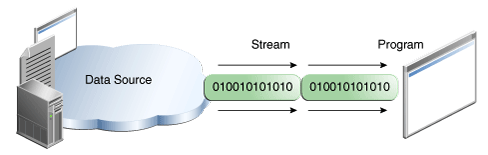
\includegraphics[width=0.45\textwidth]{images/inputstream.png}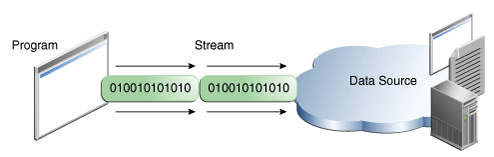
\includegraphics[width=0.45\textwidth]{images/outputstream.png}
\cite{oracle:streams}
\end{center}

The classes used to do I/O are descendants of the superclasses \texttt{InputStream} or \texttt{OutputStream}. For example, to read from a file, use a \texttt{FileInputStream}. Consider this example of reading some data and then writing it out again~\cite{oracle:streams}:

\begin{verbatim}
public class CopyFile {
    public static void main(String[] args) throws IOException {

        FileInputStream in = null;
        FileOutputStream out = null;

        try {
            in = new FileInputStream("input.txt");
            out = new FileOutputStream("output.txt");
            int c;

            while ((c = in.read()) != -1) {
                out.write(c);
            }
        } finally {
            if (in != null) {
                in.close();
            }
            if (out != null) {
                out.close();
            }
        }
    }
}
\end{verbatim}

Note that the file streams are closed inside the \texttt{finally} block, to ensure they will be closed even if something goes wrong in the input/output. 

This works, but it's really, really inefficient. Why? We are reading from the disk one character (one byte) at a time and that's really quite slow. What we'd often like to do is read a whole line at once. The above example, updated for reading a whole line:

\begin{verbatim}
public class CopyFile {
    public static void main(String[] args) throws IOException {

        BufferedReader inputStream = null;
        PrintWriter outputStream = null;

        try {
            inputStream = new BufferedReader(new FileReader("input.txt"));
            outputStream = new PrintWriter(new FileWriter("output.txt"));

            String l;
            while ((l = inputStream.readLine()) != null) {
                outputStream.println(l);
            }
        } finally {
            if (inputStream != null) {
                inputStream.close();
            }
            if (outputStream != null) {
                outputStream.close();
            }
        }
    }
}
\end{verbatim}

Here we read a whole line at a time with \texttt{readLine} rather than reading one character at a time. We also use a \texttt{BufferedReader} because we want to get buffered I/O. When we read one byte at a time, each read or write request for an individual byte results in going to the disk or network and fetching the specific byte. When we work with buffered I/O, we read a buffer (some array of data) and store it. Then when we try to read a byte we check if it's in the array we already have stored. If so, we use that value instead of going to the disk. When we reach the end of the buffer, we fill up the buffer again.

Buffered output streams mean that output is kept in a buffer and only written to disk when the buffer is full. It's possible that a program error or crash might terminate execution before the buffer is written to disk and some of the expected output will not appear. To force the buffer to output its data, you can call \texttt{flush()} on the stream. Closing the stream also has the effect of flushing the buffer.

Java also has data streams and object streams, which are used for reading/writing/storing/loading more complex things. We are not going to examine them in this course.


\section*{Programming Essay: On Problem Solving}

They key to programming is simple. Okay, maybe this is a little too ambitious to say it all breaks down to this short essay, but based on my experience, this is the way to approach programming problems:

\begin{enumerate}
\item Determine where we are (point A)
\item Determine where we're trying to go (point B)
\item Find a series of steps to get us from A to B 
\end{enumerate}

A simple example with a math problem: suppose you haven't memorized the answer to something like 12 x 13. It's a simple example, but imagine you might look at it and can't jump immediately to the answer. Other than whipping out the calculator, what can you do? Break this down into a series of problems that you know how to solve: $(12 \times 10) + (12 \times 3)$. We now have three problems $(12 \times 10$, $12 \times 3$, and then adding those two answers up). But these three problems are simpler than the original problem. Because I hate those textbooks that leave things ``as an exercise to the reader'', now we can solve $12 \times 10 = 120$; $12 \times 3 = 36$; $120 + 36 = 156$. 

We do have to know the rules of math to understand how the problem can be decomposed. 

In programming, it will be necessary to subdivide: the step you come up with might be a little bit too complicated for a computer or person to execute. So you break the items of step 3 by repeating this process: your starting position, your goal, and you break it down to a series of steps to solve step. In programming, you have to keep breaking it down until the steps are small enough for the computer to execute.

How small those steps are is a matter of what language and tools you are using. You might, for example, need to do a Fourier Transform of a signal (fancy math). If you're using an advanced language you might just write FourierTransform(signal) and that does it. Or you might have to write the transform yourself at a low level.

This is the key part that carries over regardless of programming language or problem domain. Learning the syntax of the language is another matter, however.

\bibliographystyle{alpha}
\bibliography{155}


\end{document}